% !TEX program = xelatex
%%%%%%%%%%%%%%%%%%%%%%%%%%%%%%%%%%%%%%%%%
% Beamer Presentation
% LaTeX Template
% Version 1.0 (10/11/12)
%
% This template has been downloaded from:
% http://www.LaTeXTemplates.com
%
% License:
% CC BY-NC-SA 3.0 (http://creativecommons.org/licenses/by-nc-sa/3.0/)
%
%%%%%%%%%%%%%%%%%%%%%%%%%%%%%%%%%%%%%%%%%

\documentclass{beamer}
\usepackage{tikz,lmodern,textpos,hyperref,graphicx,booktabs,appendixnumberbeamer}
\usepackage{biblatex}
\bibliography{references}
\usepackage[T1]{fontenc}
\usepackage[export]{adjustbox}
\usepackage[ddmmyyyy]{datetime}


\beamertemplatenavigationsymbolsempty

\mode<presentation>{
  \usetheme{metropolis}
  \setbeamercolor{institute in head/foot}{fg=stanfordRedText}
  \setbeamercolor*{palette tertiary}{use=structure,fg=white,bg=stanfordRed}
}
\setbeamertemplate{frame footer}{feedback:
\href{ali.alkhatib@cs.stanford.edu}{ali.alkhatib@cs.stanford.edu}
(or, like, wherever you see me)}

\title{Re--framing gig work as piecework}

\author{\textbf{Ali Alkhatib} \\
\texttt{ \href{mailto:ali.alkhatib@cs.stanford.edu}{ali.alkhatib@cs.stanford.edu} ||
         \href{http://twitter.com/_alialkhatib}{@\_alialkhatib} }}

% \institute[Stanford]{Stanford University}

\date{\usdate{\formatdate{27}{7}{2016}}}

\begin{document}

\begin{frame}
\titlepage
\end{frame}

% Notes
% Hi everyone. My name's Ali, and I want to tell you about the work on ``Cooperative Labor Markets'' that I've been doing for the past several months with a number of collaborators.

\begin{frame}{What I want from you}
``Red Teaming''
  \begin{itemize}%[<+- | alert@+>]
    \item If something doesn't make sense, push on it
    \item Try to think of counter--arguments
    \item Can't get your comment in now? email/tweet/be creative
  \end{itemize}
\end{frame}

\section{Framing}

\begin{frame}{On--demand [contract] work --- Awesome!}
  \begin{itemize}%[<+- | alert@+>]
    \item Information work
      (e.g. Innocentive, Amazon Mechanical Turk (AMT))
        \cite{bernsteinSoylent,CrowdsourcingUserStudies,paolacci2010running}
    \item Expansion from information work to other kinds of work
      (e.g. driving, cleaning, etc\dots)
        \cite{zaarlyOfficial,uberOfficial}
  \end{itemize}
\end{frame}


\begin{frame}{On--demand [contract] work --- Not so awesome?}
    \begin{itemize}[<+- | alert@+>]
      \item ``Turkers'' are being exploited for their willingness to be \textbf{transient}
        \cite{turkopticon,dynamo}
      \item This is happening in other kinds of gig work too
        \cite{leakedUber,uberSuit,uberAlgorithm}
    \end{itemize}
\end{frame}

\section{Bringing it all together}

\begin{frame}{Research themes}
  At a \textit{very} high level, all of this research has been trying to figure out ways to make on--demand work better.

  Some research questions in particular:
  \begin{itemize}[<+- | alert@+>]
    \item What are the limits of on--demand work?
                                                                      \cite{akerlof1970market,foundry}
    \item How will on--demand workers be managed?
                                                                      \cite{crowdworkFuture,uberAlgorithm}
    \item What is the future of labor advocacy?
          \\Will workers find means for empowerment? How?
                                                                      \cite{turkopticon,dynamo}
    \item \textit{More amazing questions here}
    \item \textit{This presentation is going really well, isn't it?}
  \end{itemize}
\end{frame}


\section{Making sense of new with old}

\begin{frame}{Old theories to the rescue}
  \textbf{Gig work} as \textbf{piecework}?

  Relevant for a few reasons; piecework\dots
  \begin{itemize}
    \item started in the home
    \item paid workers on a per--task basis
    \item placed workers in ambiguous statuses
  \end{itemize}
  % In fact, a lot of the stuff we've been seeing over the past \textasciitilde 15 years
  % seems to map really cleanly onto this historical practice called \textit{piecework}
\end{frame}

\begin{frame}{Old theories to the rescue}
  If we map the timeline of piecework onto the gig work timeline,
  a lot of what we've seen makes a lot of sense
  \\\textit{(maybe it was even inevitable)}
\end{frame}

\section{Overlaying timelines}

\begin{frame}{Optimizing the factory line}
  \begin{figure}
    
\includegraphics[width=0.5\linewidth]{figures/making_cars}
    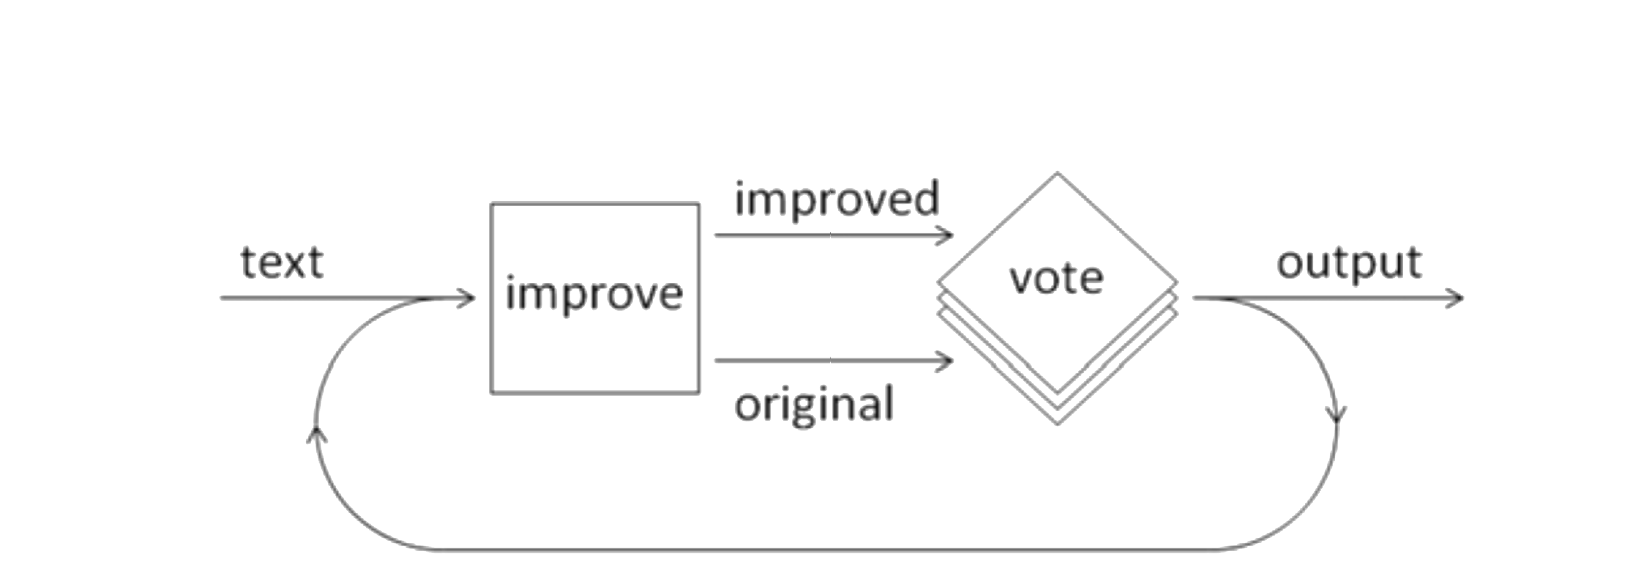
\includegraphics[width=0.5\linewidth]{figures/workflow_crowd.png}
  \end{figure}
  Research exploring how to improve the assembly line % spanning decades
  \cite{fageol1932motor,hu1961parallel}
  parallels research on crowd work--flows
  \cite[e.g.][]{weld2010decision}
\end{frame}

\begin{frame}{Disillusionment}
  \begin{figure}
    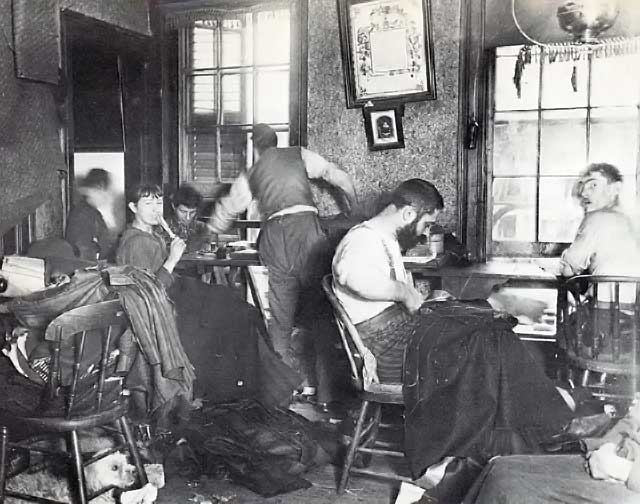
\includegraphics[width=0.43\linewidth]{figures/how_the_other_half_works.jpg}
    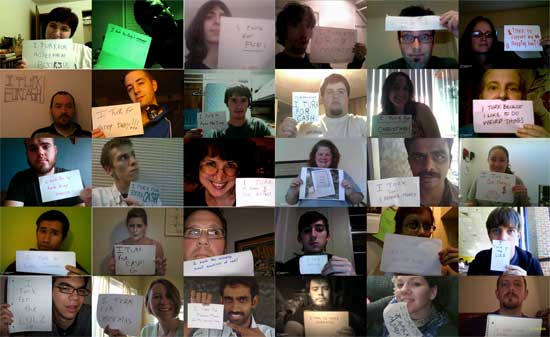
\includegraphics[width=0.57\linewidth]{figures/faces_of_mechanical_turk_small.jpg}
  \end{figure}
  \citeauthor{riisOtherSideLives} documenting pieceworkers \cite{riisOtherSideLives};
  crowdsourced documentation of ``Turkers'' \cite{facesOfMechanicalTurk}
\end{frame}

\section{Can we predict best and worst--case possibilities?}

\begin{frame}{Format}
  \begin{itemize}
    \item think about the \textbf{best case} possibilities
    \\(and the prerequisites for this outcome)
    \item think about the \textbf{worst case} possibilities
  \end{itemize}
\end{frame}

\begin{frame}{Limits of on--demand work}
  \textbf{Best case}

  We find ways to enable highly creative, perhaps even \textit{complex}, teams to do difficult tasks.
  \\Some of this is just now emerging, or in the pipeline
  \cite[see][also more of Niloufar's work]{foundry,suzukiAtelier}.

  \textbf{Worst case}

  Low--quality work (e.g. \cite{jonBrelig}) becomes the \textbf{principle} form of work for on--demand workers.
\end{frame}

\begin{frame}{Managing on--demand workers}
\textbf{Best case}

Management becomes more transparent, diminishing the need for tools like Turkopticon
\\Would require designing around rejection more carefully
\cite{takingAHITMcInnis}.

\textbf{Worst case}

Management becomes even more opaque;
maybe workers get pitted against each other in some kind of Panopticon
\cite{foucault1977discipline}.

\end{frame}

\begin{frame}{Labor advocacy's future}
\textbf{Best case}

Some form of labor advocacy emerges without the pitfalls of conventional labor unions
(which eventually alienated more junior members by appearing somewhat ossified)
\cite{ahlquist2013interest}.


\textbf{Worst case}

Workers never find lasting tools to counter exploitative labor markets
\\Would probably be the result of transient workers never being able to overcome
the barriers \citeauthor{mccallum2013global} discusses in
\cite{mccallum2013global}.
\end{frame}

\begin{frame}{Poke holes in this}
This whole thing only works because you ask hard questions,
or give me random input that may or may not be good.
\end{frame}

\begin{frame}
  \frametitle{Contact}
    name: \href{https://ali-alkhatib.com}{Ali Alkhatib} \\
    human: (Sometimes) in Gates 360 \\
    email: \href{mailto:ali.alkhatib@cs.stanford.edu}{ali.alkhatib@cs.stanford.edu} \\
    twitter: \href{https://twitter.com/_alialkhatib}{@\_alialkhatib} \\
\end{frame}

% Notes
% I'm over time [just guessing, but really], but if you have any questions, or criticism, or suggestions, I would really like to hear from you. My contact information is all there, so please approach me so we can talk in further depth about these topics - Thanks!

\begin{frame}[allowframebreaks]{References}
  \printbibliography
%   \bibliography{references}
%   \bibliographystyle{abbrv}
\end{frame}

\end{document} 